\documentclass[]{beamer}
\usepackage[T1]{fontenc}
\usepackage[utf8]{inputenc}
\usepackage{lmodern}
\usepackage[italian]{babel}

\title{Le reti di computer}
\author{Mattia Cozzi}
\date{a.f.~2024/2025}


%\documentclass[handout]{beamer}     %usare questa classe per generare l'handout

%\usepackage{pdfpages}   %per mostrare più quadri nella stessa pagina
%\pgfpagesuselayout{4 on 1}[a4paper,border shrink=5mm,landscape]


\usetheme{Singapore}
%\useoutertheme[left]{sidebar} %elementi intorno alle diapositive
\setbeamercovered{dynamic} %modifica l'aspetto del testo grigetto delle diapositive future. Argomenti: invisible/transparent/dynamic


%COLORE PRINCIPALE
\definecolor{verde}{RGB}{2, 194, 117} % UBC Blue (primary)
\setbeamercolor{structure}{fg=verde} % itemize, enumerate, etc
\setbeamercolor{alerted text}{fg=verde}


\usecolortheme{orchid}

\usepackage{tikz}

\begin{document}

\begin{frame}
  \titlepage
\end{frame}


\begin{frame}
\frametitle{Contenuti}
\tableofcontents
\end{frame}



\section{Classificazioni}


\begin{frame}
\frametitle{Collegamento}
I computer vengono collegati tra loro per:
\begin{itemize}
  \item comunicare tra loro;\pause
  \item condividere risorse:\pause
  \begin{itemize}
    \item hardware (stampanti);\pause
    \item files (su dischi fissi condivisi);\pause
    \item programmi o interi sistemi operativi;\pause
  \end{itemize}
\end{itemize}

~

Il collegamento avviene tramite un componente hardware chiamato \alert{scheda di rete}.
\end{frame}


\begin{frame}
\frametitle{Dimensione delle reti (1)}
Possiamo classificare le reti in base alla loro \alert<1>{dimensione}:\pause
\begin{description}
  \item[] Reti locali:
  \item[(W)LAN] ((Wireless) Local Area Network), terminali connessi nello stesso luogo (casa, ufficio);\pause
  \item[MAN] (Metropolitan Area Network), terminali in un'area urbana o comuni limitrofi;\pause
  \item[] Reti geografiche:
  \item[WAN] (Wide Area Network), terminali in un'intera nazione;\pause
  \item[GAN] (Global Area Network), terminali in tutti i continenti.
\end{description}
\end{frame}


\begin{frame}
  \frametitle{Dimensione delle reti (2)}
\begin{figure}
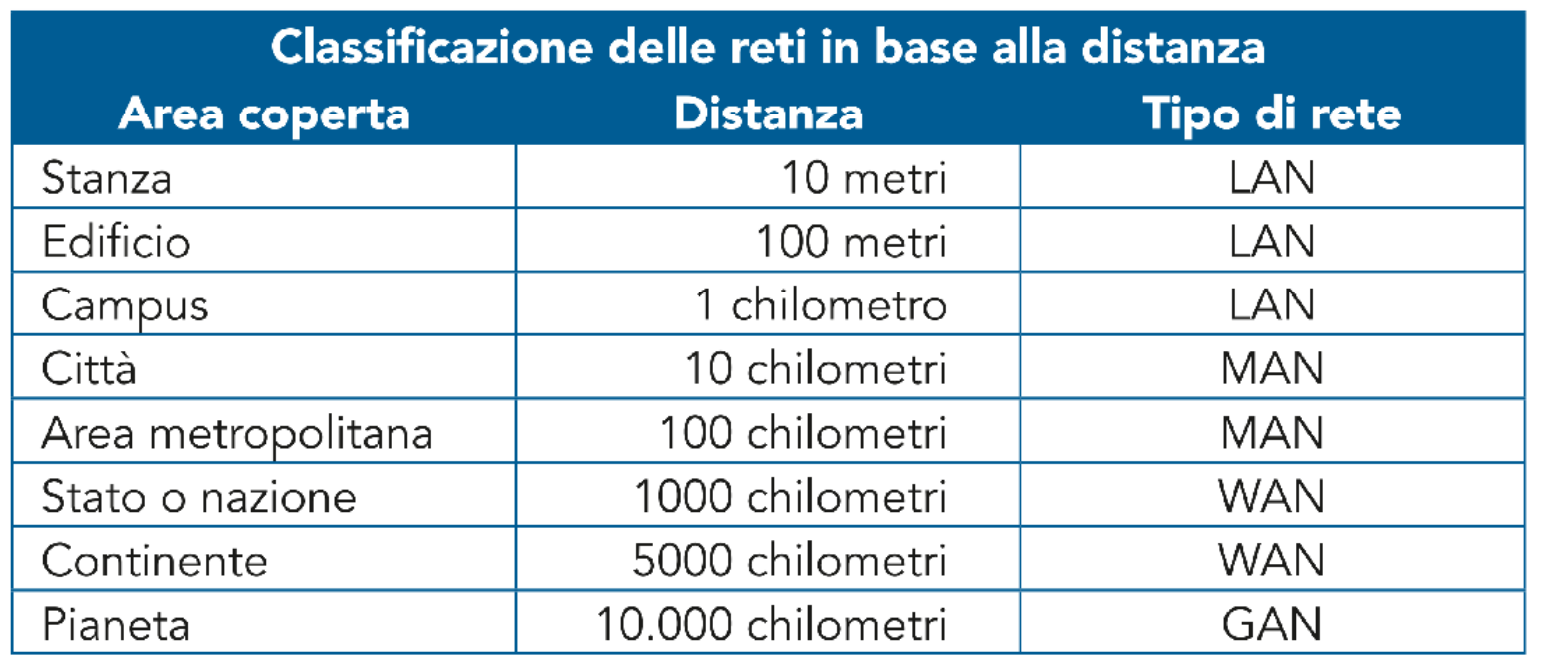
\includegraphics[width=.9\columnwidth]{img/dimensionereti.png}
\end{figure}
\end{frame}


\begin{frame}
\frametitle{Modello client/server e peer to peer}
Come avviene la condivisione di risorse?\pause

~

Dividiamo le reti in due classi:
\begin{description}
  \item[client/server] alcuni computer (server o host) mettono a disposizione risorse, altri (client) le utilizzano;\pause
  \item[peer to peer] tutti i computer condividono le loro risorse e tutti possono utilizzarle.\pause
\end{description}

~

Nel modello peer to peer ogni computer è sia server sia client.
\end{frame}


\begin{frame}
\frametitle{Schema del modello client-server}
\begin{figure}
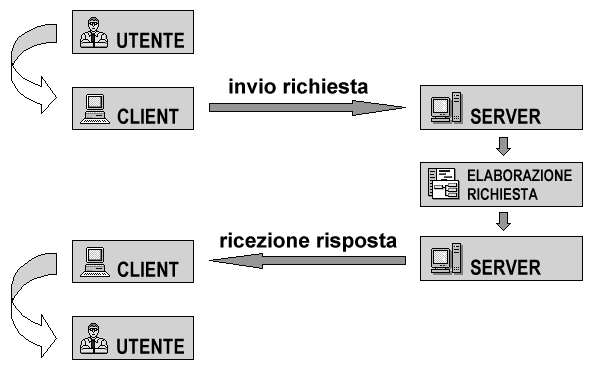
\includegraphics[width=.7\columnwidth]{screenshots/clientserver.png}
\end{figure}
\end{frame}


\section{Networking}

\begin{frame}
\frametitle{Rete aziendale}
Una rete aziendale è una rete che serve a condividere le risorse informatiche di un'azienda (files e documenti, ma anche stampanti e altro).\pause

~

È necessaria la presenza di uno \alert<2>{switch}, un dispositivo che permette di smistare il traffico di dati sui vari terminali.\pause

~

Per collegare la rete aziendale all'esterno (come alla rete internet) è necessario un \alert<3>{router}. I dati sono protetti da un \alert<3>{firewall}.\pause

~

I dispositivi connessi devono possedere ovviamente una \alert<4>{scheda di rete}.
\end{frame}



\begin{frame}
\frametitle{VPN}
Spesso le aziende (e ultimamente anche i privati) utilizzano una VPN (Virtual Private Network).\pause

~

La VPN permette di inviare dati in maniera criptata (e quindi sicura) ad un server esterno, che si interfaccia poi con la rete internet.

\visible<2->{\begin{figure}
  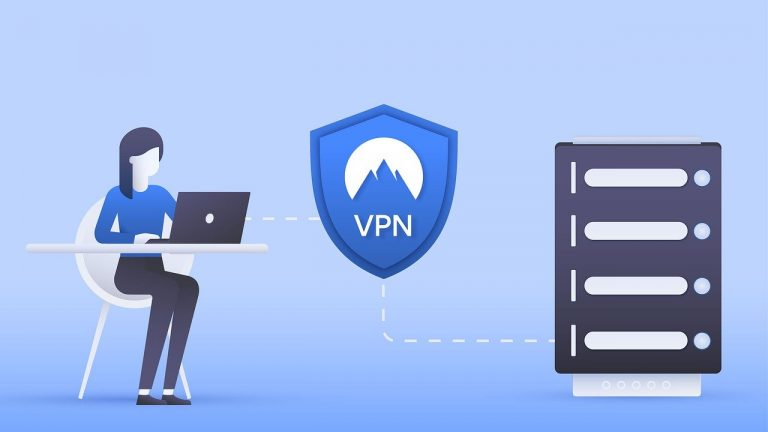
\includegraphics[width=.5\columnwidth]{img/vpn.jpg}
\end{figure}}
\end{frame}




\begin{frame}
\frametitle{Indirizzi IP}
L'indirizzo IP è composto da \alert<1>{4 cifre da 0 a 255 separate da punti} e serve a identificare in modo univoco un dispositivo in rete.
~

\begin{figure}
  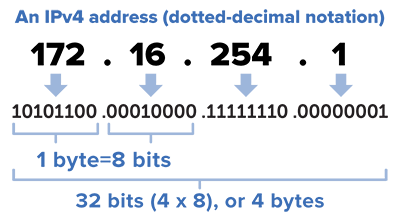
\includegraphics[width=.6\columnwidth]{img/ip.png}
\end{figure}
\end{frame}



\section{Internet}


\begin{frame}
\frametitle{Storia}
\begin{description}
  \item[1969] Il progetto ARPANET, finanziato dal Dipartimento della Difesa statunitense è la prima rete mai costruita, ottenuta collegando quattro nodi. Le applicazioni eseguite erano principalmente programmi di File Transfer Protocol (FTP).\pause
  \item[1971] Viene inventata la posta elettronica. I nodi salgono a 15, con 23 hosts.\pause
  \item[1973] Viene sviluppato il protocollo TCP/IP.\pause
  \item[1991] Tim Berners-Lee inventa il protocollo HTTP e il linguaggio HTML: nasce la rete internet moderna.\pause
  \item[1993] Nasce il primo browser, Mosaic.
\end{description}
\end{frame}

\begin{frame}
\frametitle{La prima rete}
\begin{figure}
    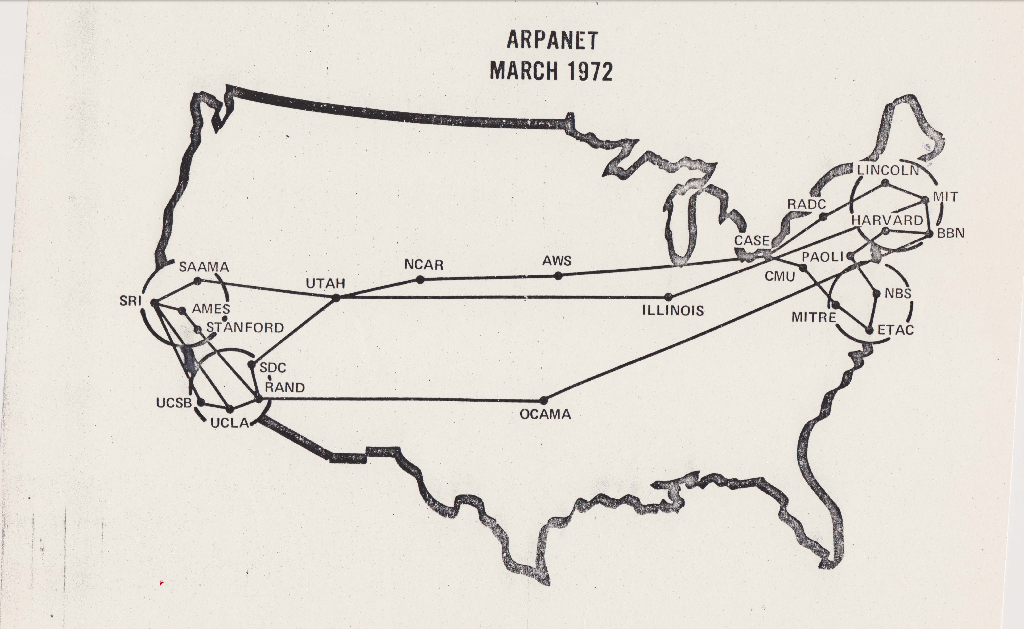
\includegraphics[width=.9\columnwidth]{img/arpanet.png}
  \end{figure}
\end{frame}


\begin{frame}
\frametitle{Una rete globale distribuita}
Un aspetto importante di Internet è la sua \alert<1>{topologia distribuita e decentrata}: è formata dall'integrazione di numerose sottoreti pubbliche, commerciali e private.\pause

~

Se un percorso è interrotto o troppo trafficato i dati possono prendere strade alternative.

~

\begin{figure}
  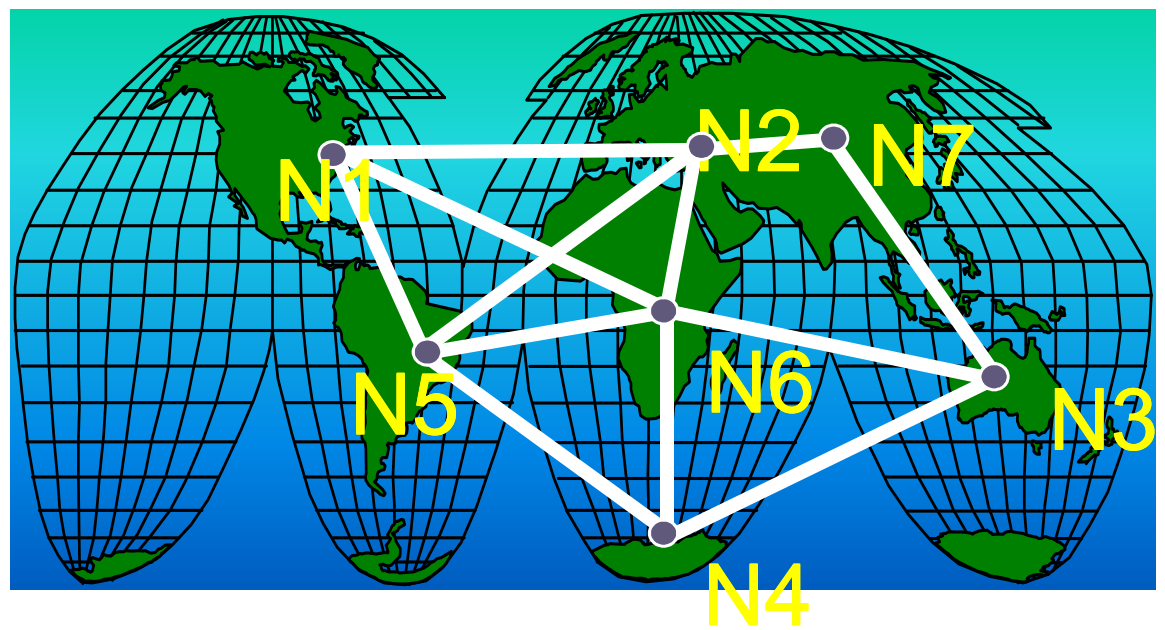
\includegraphics[width=.5\columnwidth]{img/percorsi.png}
\end{figure}
\end{frame}




\begin{frame}
\frametitle{Il web}
Il \alert<1->{World Wide Web} (WWW) è il principale servizio di internet: è l'insieme dei documenti (pagine web o altro) collegati tra loro.\pause

~

Il collegamento avviene mediante \alert<2>{hyperlinks} (o links, o collegamenti ipertestuali).\pause

~

Le pagine web sono particolari tipi di documenti chiamati \alert<3>{ipertesti} e sono scritte in linguaggio HTML (HyperText Markup Language).
\end{frame}


\begin{frame}
\frametitle{Indirizzi}
Ogni risorsa è identificata da un \alert<1>{indirizzo} (URL, uniform resource locator). Un semplice esempio:\pause

\begin{center}
  \visible<2->{\alert<2>{\texttt{https://}}}\visible<3->{\alert<3>{\texttt{www.}}}\visible<4->{\alert<4>{\texttt{google}}}\visible<5->{\alert<5>{\texttt{.it}}}
\end{center}

~

Un indirizzo contiene:
\begin{itemize}
  \item un \alert<2>{protocollo} (come \texttt{http} o \texttt{https}, più sicuro);\pause
  \item l'indicazione del \alert<3>{servizio} (come \texttt{www} per il web);\pause
  \item un \alert<4>{dominio di secondo livello} (cioè il nome della risorsa, sito);\pause
  \item un \alert<5>{dominio di primo livello} (come \texttt{.it} o \texttt{.com}).\pause
\end{itemize}

~

Gli URL sono in realtà costituti da indirizzi IP, associati ad un testo da un DNS (Domain Name System).
\end{frame}


\begin{frame}
\frametitle{Navigare in rete: il browser}
Per visualizzare le risorse presenti online (come i siti web) è necessario un \alert<1>{browser} (letteralmente ``sfogliatore''), che permette di \alert<1>{navigare in internet}.

~

\begin{figure}
  
\includegraphics[width=.7\columnwidth]{img/browsers.png}
\end{figure}\pause

~

Quando visualizziamo una pagina, l'utente digita un URL, il browser la richiede al server. Se il server risponde positivamente, fornisce la risorsa al browser, che la mostra all'utente.
\end{frame}



\end{document}
